\documentclass[11pt]{article}

%==============================================================
% OICC: Over-Identification-Calibrated Conformal Deconvolution
%==============================================================

\usepackage[utf8]{inputenc}
\usepackage[T1]{fontenc}
\usepackage{amsmath,amssymb,amsthm}
\usepackage{mathtools}
\usepackage{bm}
\usepackage{booktabs}
\usepackage{array}
\usepackage{graphicx}
\usepackage{xcolor}
\usepackage[margin=1in]{geometry}
\usepackage[hidelinks]{hyperref}
\usepackage[ruled,vlined]{algorithm2e}
\usepackage{caption}
\usepackage{enumitem}

%--------------------------------------------------------------
% Theorem environments
%--------------------------------------------------------------
\newtheorem{theorem}{Theorem}
\newtheorem{proposition}{Proposition}
\newtheorem{lemma}{Lemma}
\newtheorem{corollary}{Corollary}
\theoremstyle{definition}
\newtheorem{assumption}{Assumption}
\newtheorem{definition}{Definition}
\theoremstyle{remark}
\newtheorem{remark}{Remark}

%--------------------------------------------------------------
% Notation macros
%--------------------------------------------------------------
\newcommand{\Var}{\operatorname{Var}}
\newcommand{\Cov}{\operatorname{Cov}}
\newcommand{\E}{\mathbb{E}}
\newcommand{\R}{\mathbb{R}}
\newcommand{\btheta}{\bm{\theta}}
\newcommand{\thh}{\widehat{\theta}}
\newcommand{\eps}{\varepsilon}
\newcommand{\dperp}{\Delta_{\perp}}
\newcommand{\dpar}{\Delta_{\parallel}}
\newcommand{\Yc}{Y^{c}}

\title{\bf Over-Identification-Calibrated Conformal Deconvolution:\\
Honest Latent-Rate Estimation from Multiple Biased\\ Institutional Records}

\author{%
Anonymous Submission%
}

\date{}

\begin{document}
\maketitle

%==============================================================
\begin{abstract}
%==============================================================
Administrative records of social harms---recorded crime, distress calls,
complaints, accountability filings---are not the harm itself. Each is a
biased, mechanism-specific measurement of a latent rate that is
\emph{never observed}. We present OICC (Over-Identification-Calibrated
Conformal Deconvolution), a method that estimates a latent per-area-period
rate $\theta$ from $K\ge 3$ mechanism-independent noisy channels under a
one-factor measurement model, and---critically---quantifies how much of
its own answer is defensible. OICC composes four ingredients that are
individually known but, to our knowledge, have not been assembled into an
end-to-end, self-auditing estimator: (i) closed-form tetrad moment
identification of factor loadings and $\Var(\theta)$;
(ii) a \emph{loading-invariant over-identification specification test}
that detects departures from the one-factor law in directions orthogonal
to the shared signal (bootstrap Wald, $\mathrm{df}=K(K-1)/2-K$); (iii) a
novel \emph{leave-pivot-out conformal} primitive giving both an
exact finite-sample distribution-free interval for an observed channel
value and a model-assisted asymptotic interval for the latent $\theta$;
and (iv) an explicit \emph{impossibility/escape} pairing: we prove that a
common-mode confounder loaded along the signal direction is unidentified
by \emph{any} over-ID test at \emph{any} $K$, and show that $Q\ge 2$
negative-control (proximal) channels \emph{point-identify} $\Var(\theta)$
when available, with honestly untestable assumptions. Around this core we
add three deployment-grade tools: an \emph{exclusion-sensitivity} analysis
that reports the bounded band of $\Var(\theta)$ implied by a violation of
the negative-control exclusion restriction (a Cinelli--Hazlett-flavored
bounded-bias sweep with a robustness value $\eps^\star$), directly answering
the standard objection that exclusion is untestable; an \emph{anytime-valid
deployment monitor} that runs a Vovk--Wang $p$-to-$e$ calibrated product
e-process over the stream of per-period over-ID $p$-values and, by Ville's
inequality, controls the time-uniform false-alarm rate; and \emph{bootstrap}
(i.i.d.\ and moving-block) uncertainty quantification on every estimator.
On synthetic ground truth the over-ID test attains
size $\le 0.05$ and power $\approx 1.00$ against detectable confounders and
provably $0.00$ against common-mode confounders; observed-value coverage is
exact ($0.90$) and latent coverage is $\approx 0.89$; proximal
point-identification holds $\Var(\theta)$ at the truth $0.61$ across
common-mode strengths $\{0,0.5,1.0,1.5,2.0\}$ where the naive estimate
inflates to $\{0.61,0.77,1.25,2.05,3.18\}$, with bootstrap CIs covering truth;
the exclusion-sensitivity band collapses to the point estimate at zero
violation, widens with it, and contains the true $\Var(\theta)$ under a known
injected violation; and the monitor holds an anytime false-alarm rate of
$0.013\le0.05$ over long null streams while detecting a structural drift with
median delay $\approx 9$ windows. On India NCRB state-year data (2001--2010,
$N{=}253$, four institutional channels) the one-factor law is not rejected in
detectable directions ($p{=}0.088$); as a two-directional check of the
specification test, a cross-national run on real Chicago and NYC data
(2018--2023) treating the three crime \emph{categories} as shared-filter
pseudo-channels is correctly \emph{rejected} ($p<0.001$). We make no
claim of distribution-free finite-sample \emph{latent} coverage---which we
prove is impossible---only exact coverage for observed values and
asymptotic coverage for the latent rate.
\end{abstract}

%==============================================================
\section{Introduction}\label{sec:intro}
%==============================================================

\paragraph{Records are not truth.}
Suppose we want the true rate of a social harm---criminal victimization,
domestic violence, custodial abuse---in an area during a period. We do not
observe it. We observe \emph{institutional records}: crimes police chose to
register, emergency calls citizens chose to place, complaints that were
filed, accountability proceedings that were opened. Each record-generating
process has its own gate: reporting propensity, registration incentives,
capacity, and trust in the institution. Every channel is therefore a
\emph{biased} measurement of the same underlying quantity, and the bias is
neither known nor observed. Naively treating any single channel---or a
simple average---as ``the rate'' conflates the harm with the machinery that
records it, a conflation with direct consequences for resource allocation
and for fairness audits of the institutions themselves.

\paragraph{The latent-rate problem.}
We formalize the target as a latent per-area-period rate $\theta$ measured
by $K \ge 3$ channels through a one-factor model
$Y^c = \alpha_c + \beta_c\,\theta + \eps^c$, with channel errors mutually
independent given $\theta$. Two facts make this hard and interesting. First,
$\theta$ is \emph{never} observed, so we can never directly validate a
point estimate or an interval on real data. Second, honesty about
\emph{what cannot be known} is as important as the estimate: a method that
silently reports a tight interval around a confounded quantity is worse than
useless in a policy or fairness setting.

\paragraph{Contributions.}
Our contribution is a \emph{composition} and one new primitive, not a claim
to have invented factor analysis, deconvolution, or conformal prediction.
Specifically:
\begin{enumerate}[leftmargin=1.6em,itemsep=2pt]
\item \textbf{A self-auditing estimator (OICC).} We assemble closed-form
tetrad identification, an over-identification specification test, a
conformal calibration layer, and a proximal escape hatch into a single
pipeline whose output includes a certificate of what it can and cannot
defend (Sec.~\ref{sec:method}).
\item \textbf{Leave-pivot-out latent conformal (new primitive).} We hold out
one ``pivot'' channel, predict it via the best linear unbiased predictor
(BLUP) from the others, and exploit that the prediction residual splits as
$R = S + \eps^{\text{pivot}}$ with $S \perp \eps^{\text{pivot}}$
\emph{by construction}. This yields (a) an \emph{exact} finite-sample
distribution-free split-conformal interval for the observed pivot value and
(b) a model-assisted asymptotic interval for the latent $\theta$ obtained by
deconvolving the known law of $S$ (Sec.~\ref{sec:conformal}).
\item \textbf{A loading-invariant over-ID test.} Working in
$\log|\Cov(Y^j,Y^k)|$ turns the rank-one covariance restriction into an
additive two-way model whose residuals are exactly the over-identifying
restrictions, giving a test that is \emph{invariant to the (unknown)
loadings} (Sec.~\ref{sec:overid}).
\item \textbf{An honest impossibility/escape pairing.} We prove that a
common-mode confounder loaded along $\beta$ is invisible to any over-ID test
at any $K$ and unidentified from the observed covariance, and we show that
$Q\ge 2$ negative-control channels \emph{point-identify} $\Var(\theta)$ under
explicit, \emph{untestable} assumptions (Sec.~\ref{sec:impossible}). Bootstrap
CIs (i.i.d.\ and moving-block) accompany every estimate.
\item \textbf{Deployment-grade honesty tooling.} We add (a) an
\emph{exclusion-sensitivity} analysis that bounds the effect of violating the
negative-control exclusion restriction and reports a robustness value
$\eps^\star$, directly addressing the objection that exclusion is untestable
(Sec.~\ref{sec:exclusion}); and (b) an \emph{anytime-valid deployment monitor}
---a calibrated e-process over the stream of over-ID $p$-values that controls
the time-uniform false-alarm rate by Ville's inequality
(Sec.~\ref{sec:monitor}). We validate the specification test in
\emph{both} directions: it does not reject institutionally-independent India
channels ($p{=}0.088$) but does reject US crime categories that share one
recording filter ($p<0.001$), Sec.~\ref{sec:us}.
\end{enumerate}

We deliberately do not overclaim. In particular we never assert
distribution-free finite-sample coverage of the \emph{latent} rate; we prove
that is impossible (Sec.~\ref{sec:impossible}) and report only exact coverage
for observed values plus asymptotic coverage for $\theta$.

%==============================================================
\section{Related Work and Exact Deltas}\label{sec:related}
%==============================================================

OICC lives at the intersection of measurement-error deconvolution,
proximal causal inference, and conformal prediction. We name the closest
prior art and state precisely what we add.

\paragraph{Deconvolution and latent-factor identification.}
Kotlarski's identity \cite{kotlarski1967} identifies the distribution of a
latent variable from two independent noisy measurements; Li and Vuong
\cite{livuong1998} give an empirical-characteristic-function estimator, and
Delaigle, Hall and Meister \cite{dhm2008} analyze repeated-measurement
deconvolution rates. Hu and Schennach \cite{huschennach2008} establish
nonparametric identification of nonclassical measurement-error models.
\emph{Delta:} these works identify or estimate the latent \emph{law}; none
provides a \emph{specification test} for the measurement model, a
finite-sample interval for a held-out channel, or a self-audit of when the
whole model is confounded. We reuse the moment identity but add the over-ID
test and conformal layer on top.

\paragraph{Proximal / negative-control inference.}
Kuroki and Pearl \cite{kurokipearl2014} and Miao, Geng and Tchetgen Tchetgen
\cite{miao2018} show that pairs of ``negative control'' proxies identify
causal effects in the presence of unmeasured confounding.
\emph{Delta:} we import their negative-control machinery specifically as the
\emph{escape hatch} for the common-mode blind spot we prove OICC otherwise
has, and we are explicit that their completeness/exclusion conditions are
untestable in our setting.

\paragraph{Conformal prediction.}
Romano, Patterson and Cand\`es \cite{romano2019cqr} give conformalized
quantile regression; Jin, Ren and Cand\`es \cite{jin2023} conformalize under
covariate/label shift; Angelopoulos et al.\ \cite{ppi} (prediction-powered
inference) and Chugg et al.\ \cite{chugg2023} give valid inference combining
predictions with a small labeled sample. \emph{Delta:} all of these assume
access to some observed outcome (labels, or an anchoring sample). Our target
$\theta$ is \emph{never} observed. Our leave-pivot-out construction manufactures
an observed surrogate---a held-out channel---so that split conformal applies
to it exactly, and then transports calibration to the latent scale via a
\emph{known} error law rather than any labeled $\theta$.

\paragraph{Sensitivity analysis and anytime-valid inference.}
Cinelli and Hazlett \cite{cinelli2020} formalize omitted-variable bias as a
bounded sensitivity problem with an interpretable \emph{robustness value};
Shi, Miao and Tchetgen Tchetgen \cite{shi2020} review negative-control /
proximal designs. On the sequential side, Ramdas et al.\ \cite{ramdas2023}
survey game-theoretic anytime-valid inference, Waudby-Smith and Ramdas
\cite{wsr2024} construct e-values and confidence sequences for bounded means,
and Chugg et al.\ \cite{chugg2023} give sequential prediction-powered
inference. \emph{Delta:} we do not develop new sensitivity or e-process
theory. We \emph{compose} them into OICC as two honesty tools: a bounded
exclusion-violation sweep (Cinelli--Hazlett-flavored, but over the
negative-control exclusion restriction rather than a regression coefficient)
that yields a $\Var(\theta)$ band and a robustness value $\eps^\star$, and a
Vovk--Wang $p$-to-$e$ product e-process over the stream of over-ID $p$-values
that monitors a deployed model with a time-uniform false-alarm guarantee.
Neither the exclusion violation's sign nor the analyst's maximal tolerated
violation $\eps_{\max}$ is estimable; we treat them as an explicit expert
prior, which is exactly the honest posture the objection demands.

\paragraph{Small-area and ecological estimation.}
Manrique-Vallier and collaborators \cite{manriquevallier} model latent
population structure for multiple-systems (capture--recapture) estimation.
\emph{Delta:} we do not assume list/capture structure; our channels are
biased continuous measurements, and our emphasis is on \emph{testable
falsification} of the measurement model plus honest reporting of the
unidentified direction.

\paragraph{Our position.}
None of the individual primitives is new. The contribution is the
\emph{end-to-end composition}, the \emph{leave-pivot-out latent conformal}
primitive, and the \emph{explicit pairing of a proven impossibility with a
proximal escape}, so that a practitioner receives not just $\thh$ but a
statement of what is and is not defensible.

%==============================================================
\section{Method}\label{sec:method}
%==============================================================

\subsection{Measurement model}\label{sec:model}

Index areas--periods (units) by $i=1,\dots,N$ and channels by
$c=1,\dots,K$.

\begin{assumption}[One-factor measurement model]\label{ass:onefactor}
For each unit $i$ and channel $c$,
\begin{equation}\label{eq:model}
Y^{c}_i \;=\; \alpha_c + \beta_c\,\theta_i + \eps^{c}_i,
\qquad
\eps^{c}_i \mid \theta_i \;\text{ mutually independent across } c,
\end{equation}
with $\E[\eps^c_i\mid\theta_i]=0$ and finite second moments. The scale is
fixed by the pivot normalization $\beta_1 = 1$.
\end{assumption}

Assumption~\ref{ass:onefactor} says the channels share \emph{exactly one}
common driver $\theta$ and that, conditional on it, their idiosyncratic
errors (reporting noise, registration noise, capacity noise) are
independent. The normalization $\beta_1=1$ makes $\theta$ interpretable on
the scale of channel 1 (the pivot); it is a labeling choice, not an
assumption.

\subsection{Moment identification via tetrads}\label{sec:ident}

Under \eqref{eq:model}, for $j \ne k$ the off-diagonal covariances carry no
error contamination:
\begin{equation}\label{eq:cov}
\Cov(Y^j, Y^k) \;=\; \beta_j\,\beta_k\,\Var(\theta).
\end{equation}
The diagonal $\Var(Y^c)=\beta_c^2\Var(\theta)+\Var(\eps^c)$ is contaminated
by error and is \emph{not} used for loading identification. From
\eqref{eq:cov}, ratios of covariances give the loadings and, together with
$\beta_1=1$, the factor variance. With $K\ge 4$ the same $\Var(\theta)$ is
implied by multiple \emph{tetrads}
$\Cov(Y^j,Y^k)\Cov(Y^l,Y^m) = \Cov(Y^j,Y^l)\Cov(Y^k,Y^m)$, and we take a
covariance-weighted average of the closed-form solutions.

\begin{proposition}[Closed-form identification]\label{prop:ident}
Under Assumption~\ref{ass:onefactor} with $K \ge 3$ and $\beta_c \ne 0$,
$\Var(\theta)$ and $\{\beta_c\}$ are identified from the off-diagonal
covariance matrix by
\[
\beta_j\beta_k = \frac{\Cov(Y^j,Y^k)}{\Var(\theta)},\quad
\Var(\theta) = \frac{\Cov(Y^1,Y^j)\Cov(Y^1,Y^k)}{\Cov(Y^j,Y^k)}\ \text{(for } j,k\ne 1),
\]
and are \emph{over-identified} for $K\ge 4$. Estimators substitute sample
covariances and average across tetrads.
\end{proposition}

\subsection{Loading-invariant over-identification test}\label{sec:overid}

The rank-one structure \eqref{eq:cov} implies a multiplicative constraint on
the $\binom{K}{2}$ off-diagonal covariances. Taking logs of absolute values
linearizes it:
\begin{equation}\label{eq:logadd}
\log\bigl|\Cov(Y^j,Y^k)\bigr| \;=\; a_j + a_k + c,
\qquad a_c := \log|\beta_c|,\ \ c := \log\Var(\theta),
\end{equation}
an \emph{additive two-way (rank-one) model} in $(j,k)$. Crucially, the
residuals of \eqref{eq:logadd}---the amount by which the observed
log-covariances fail to be additive---are exactly the over-identifying
restrictions, and they \emph{do not depend on the unknown loadings}: fitting
\eqref{eq:logadd} absorbs the $a_c$. This is what we mean by a
\emph{loading-invariant} test.

\begin{definition}[Over-ID statistic]\label{def:overid}
Let $r_{jk}$ be the residuals from the least-squares fit of
\eqref{eq:logadd}. The over-ID statistic is the bootstrap Wald quantity
$T = \hat r^\top \widehat{\Sigma}_r^{+}\, \hat r$ with degrees of freedom
\[
\mathrm{df} \;=\; \binom{K}{2} - K \;=\; \frac{K(K-1)}{2} - K,
\]
where $\widehat{\Sigma}_r$ is a nonparametric bootstrap covariance of the
residual vector and ${}^{+}$ denotes pseudo-inverse.
\end{definition}

At $K=3$, $\mathrm{df}=0$: the one-factor model is \emph{just} identified and
the covariance test has no power. In that case OICC falls back to a
third-cumulant restriction (skewness co-moments), which we \emph{flag as
low power} and never present as a substitute for the $K\ge 4$ test.

\begin{proposition}[What the test can and cannot see]\label{prop:power}
Write a candidate confounder's loading vector as $\delta = \dperp + \dpar$,
where $\dpar$ is the component parallel to the signal loading $\beta$ and
$\dperp$ is orthogonal. The over-ID residuals in \eqref{eq:logadd} are a
function of $\dperp$ only; they are identically zero for any $\dpar$.
Consequently the test has (asymptotic) power against $\dperp\ne 0$ and
\emph{exactly zero} power against $\dpar$.
\end{proposition}

Proposition~\ref{prop:power} is the formal statement of the blind spot we
confront head-on in Sec.~\ref{sec:impossible}: a purely common-mode
confounder is undetectable, by construction, not by weakness of the test.

\subsection{Two-interval leave-pivot-out conformal}\label{sec:conformal}

We now build calibrated uncertainty. Designate channel 1 the \emph{pivot}.
Using only the \emph{non-pivot} channels $\{2,\dots,K\}$ and the identified
moments, form the BLUP of the pivot's signal,
$\thh_i = \E_{\text{lin}}[\theta_i \mid Y^2_i,\dots,Y^K_i]$ (equivalently a
predictor of $\beta_1\theta_i=\theta_i$). Define the pivot residual
\begin{equation}\label{eq:resid}
R_i \;=\; Y^1_i - \thh_i \;=\; \underbrace{(\theta_i - \thh_i)}_{=:S_i} + \eps^{1}_i .
\end{equation}

\begin{lemma}[By-construction independence]\label{lem:indep}
Because $\thh_i$ is a function of $Y^2,\dots,Y^K$ only, and $\eps^1$ is
independent of $(\theta,\eps^2,\dots,\eps^K)$ under
Assumption~\ref{ass:onefactor}, the two terms in \eqref{eq:resid} are
independent: $S_i \perp \eps^1_i$. Moreover
$\Var(S) = \Var(R) - \Var(\eps^1)$, and $\Var(\eps^1)$ is identified from the
moment identity ($\Var(Y^1)-\beta_1^2\Var(\theta)$).
\end{lemma}

This clean split powers two \emph{nested} intervals.

\paragraph{Interval 1: exact, distribution-free, for the observed pivot.}
The residuals $\{R_i\}$ are exchangeable calibration scores for predicting
the observed value $Y^1$. Standard split conformal on $\{R_i\}$ therefore
yields a prediction interval for a new $Y^1_{\text{new}}$ with
\emph{finite-sample, distribution-free} coverage $\ge 1-\alpha$. This makes
no use of \eqref{eq:model} beyond exchangeability.

\paragraph{Interval 2: model-assisted, asymptotic, for the latent $\theta$.}
We want an interval for $\theta_{\text{new}}$, not $Y^1_{\text{new}}$. Since
$\theta_{\text{new}} = \thh_{\text{new}} + S_{\text{new}}$ and the law of $S$
is \emph{known} (its variance is identified by Lemma~\ref{lem:indep}, and $S$
is a near-Gaussian average of many channel errors by a CLT across channels),
we invert the known law of $S$ around $\thh_{\text{new}}$. For heavy-tailed
errors we replace the Gaussian step with characteristic-function (CF)
deconvolution of $S$ from $R$ using
$\varphi_S = \varphi_R / \varphi_{\eps^1}$.

\begin{theorem}[Coverage guarantees]\label{thm:coverage}
Under exchangeability of $\{R_i\}$, Interval 1 covers $Y^1_{\text{new}}$ with
probability $\ge 1-\alpha$ in finite samples, distribution-free. Under
Assumption~\ref{ass:onefactor} and consistency of the identified moments,
Interval 2 covers $\theta_{\text{new}}$ with probability $\to 1-\alpha$ as
$N\to\infty$. No finite-sample distribution-free guarantee for
$\theta_{\text{new}}$ exists (Theorem~\ref{thm:impossible}).
\end{theorem}

We stress the asymmetry: Interval 1 is a theorem about an \emph{observable};
Interval 2 is an asymptotic statement that \emph{relies on the model} and is
therefore only as good as the model, which is exactly why the over-ID test
and the sensitivity analysis below are not optional decorations.

\subsection{Sensitivity analysis}\label{sec:sensitivity}

OICC turns the over-ID diagnostic into calibration. Let $\widehat{\dperp}$ be
the estimated orthogonal confounder magnitude implied by the over-ID
residuals. We inflate the latent interval (Interval 2) by propagating
$\widehat{\dperp}$ into $\Var(S)$, giving a \emph{data-driven} widening that
grows with detected misspecification. For the undetectable common-mode
direction we expose a single user knob $\gamma_{\text{cm}}\ge 0$ encoding an
assumed common-mode strength; the interval widens visibly and monotonically
in $\gamma_{\text{cm}}$. This makes the blind spot \emph{operational}: the
analyst must state a common-mode assumption to obtain a tight interval, and
the report records it.

\paragraph{Bootstrap uncertainty quantification.}
All point estimates---loadings, $\Var(\theta)$, the over-ID statistic, and the
proximal point-ID estimate---are accompanied by nonparametric bootstrap
confidence intervals. For i.i.d.\ units we resample units with replacement; for
serially dependent panels (e.g.\ state-year or city-year streams) we use a
\emph{moving-block} bootstrap that resamples contiguous blocks to preserve
short-range temporal dependence. The same bootstrap covariance feeds the
over-ID Wald statistic (Def.~\ref{def:overid}).

\begin{algorithm}[t]
\caption{OICC: Over-Identification-Calibrated Conformal Deconvolution}
\label{alg:oicc}
\DontPrintSemicolon
\KwIn{Channel matrix $Y \in \R^{N\times K}$; level $\alpha$; optional
negative controls $N\in\R^{N\times Q}$; common-mode knob $\gamma_{\text{cm}}$.}
\KwOut{$\thh$; observed-value interval; latent interval; over-ID
certificate.}
\BlankLine
Estimate off-diagonal covariances; recover $\{\beta_c\}$, $\Var(\theta)$ by
averaged tetrads (Prop.~\ref{prop:ident}).\;
\If{$K \ge 4$}{
  Fit additive model \eqref{eq:logadd}; bootstrap Wald $T$,
  $\mathrm{df}=K(K-1)/2-K$; record $p$-value and $\widehat{\dperp}$
  (Def.~\ref{def:overid}).\;
}\Else{
  Third-cumulant fallback; \textbf{flag low power}.\;
}
\If{negative controls provided}{
  Residualize signal channels on controls to remove common mode
  (Sec.~\ref{sec:proximal}).\;
}
Choose pivot; compute BLUP $\thh$ from non-pivot channels; residuals $R$
\eqref{eq:resid}.\;
\textbf{Interval 1:} split conformal on $\{R_i\}$ $\Rightarrow$ exact interval
for $Y^1_{\text{new}}$.\;
\textbf{Interval 2:} deconvolve $S$ from $R$ (Gaussian or CF); invert around
$\thh$ $\Rightarrow$ latent interval.\;
Inflate Interval 2 by $\widehat{\dperp}$ and $\gamma_{\text{cm}}$
(Sec.~\ref{sec:sensitivity}).\;
\Return $\thh$, intervals, and certificate $\{p, \widehat{\dperp},
\gamma_{\text{cm}}, \text{fallback flags}\}$.\;
\end{algorithm}

%==============================================================
\section{Impossibility and the Proximal Escape}\label{sec:impossible}
%==============================================================

\subsection{The common-mode impossibility}

Consider a confounder $W$ that enters \emph{every} channel with loading
proportional to the signal loading: $Y^c = \alpha_c + \beta_c\theta +
\kappa\,\beta_c W + \eps^c$ for a common scalar $\kappa$. Collecting terms,
$Y^c = \alpha_c + \beta_c\,F + \eps^c$ with $F := \theta + \kappa W$.

\begin{theorem}[Common-mode unidentifiability]\label{thm:impossible}
If a confounder loads proportionally to $\beta$, the observable law is
\emph{exactly} a one-factor model in $F = \theta + \kappa W$. Hence
$\Var(\theta)$ is not a function of the observed covariance matrix and is
unidentified, and the over-ID residuals \eqref{eq:logadd} are identically
zero at every $K$. No over-identification test can detect this confounding,
and no finite-sample distribution-free interval for $\theta$ exists.
\end{theorem}

Theorem~\ref{thm:impossible} is not a limitation of OICC's test; it is a
property of the observable distribution. A method that reported a tight
interval here would be reporting an interval for $F$, not $\theta$, while
labeling it $\theta$. OICC instead surfaces the issue and either widens via
$\gamma_{\text{cm}}$ or escapes via negative controls.

\subsection{Escape via negative controls (proximal inference)}\label{sec:proximal}

Suppose we can find channels that carry $W$ but \emph{not} $\theta$:
\begin{equation}\label{eq:nc}
N^{q} \;=\; a_q + m_q\,W + \nu^{q}, \qquad q=1,\dots,Q,
\end{equation}
with $\nu^q$ independent of $\theta$ and $\eps$. These are
\emph{negative-control} outcomes in the sense of \cite{kurokipearl2014,miao2018}.
Residualizing the signal channels on the controls removes the common mode.

\begin{proposition}[Proximal identification]\label{prop:proximal}
Under \eqref{eq:nc} with the standard completeness/relevance conditions of
proximal inference, $Q \ge 2$ negative controls point-identify
$\Var(\theta)$ and the loadings after residualization; $Q=1$ permits
detection of the common mode and partial correction but not full
point-identification.
\end{proposition}

\begin{remark}[Honesty about assumptions]
The exclusion restriction ``$N^q$ does not depend on $\theta$'' and the
completeness conditions are \emph{untestable} from the observed data. We
therefore treat proximal correction as an assumption-laden option, reported
alongside the naive estimate, never as a silent default.
\end{remark}

\subsection{Exclusion-sensitivity analysis}\label{sec:exclusion}

The single sharpest objection to any negative-control design is that the
exclusion restriction in \eqref{eq:nc}---that the controls carry $W$ but
\emph{not} $\theta$---is untestable. Rather than assert it, we \emph{bound the
consequence of its failure}. Following the bounded omitted-variable-bias logic
of Cinelli and Hazlett \cite{cinelli2020}, we parameterize a violation by a
single scalar $\eps\in[0,\eps_{\max}]$: the fraction of a control's systematic
variance that is in fact driven by $\theta$. At $\eps=0$ the exclusion holds
and proximal point-identification (Prop.~\ref{prop:proximal}) is exact; as
$\eps$ grows, a fraction $\eps$ of the control signal leaks $\theta$ into the
residualization and biases $\Var(\theta)$. Because the sign of the leak is
itself unidentified, we sweep \emph{both} signs and report the resulting
interval
\begin{equation}\label{eq:exclband}
\mathcal{B}(\eps) \;=\; \Bigl[\, \widehat{\Var}(\theta)\big|_{-\eps},\ \
\widehat{\Var}(\theta)\big|_{+\eps} \,\Bigr],
\end{equation}
the \emph{exclusion-sensitivity band}, together with a \emph{robustness value}
$\eps^\star$: the smallest violation at which a qualitative conclusion (e.g.\
``the common mode inflates $\Var(\theta)$'') would flip.

\begin{remark}[What is and is not estimable]
The band $\mathcal{B}(\eps)$ is a \emph{bounded-bias} object, not a confidence
set: $\eps_{\max}$ is an expert prior on the maximal tolerable exclusion
violation and the violation's sign is unidentified. We therefore report the
whole curve $\eps\mapsto\mathcal{B}(\eps)$ and $\eps^\star$, letting the reader
supply their own $\eps_{\max}$, rather than collapsing to a single number.
\end{remark}

\subsection{Anytime-valid deployment monitor}\label{sec:monitor}

A model that passes the over-ID test at deployment can drift out of
specification later. We monitor a deployed OICC model over a stream of periods
$t=1,2,\dots$ by feeding the per-period over-ID $p$-value $p_t$ through a
Vovk--Wang $p$-to-$e$ calibrator $e_t = f(p_t)$ and forming the running product
e-process $M_T = \prod_{t\le T} e_t$. Under the null (structure holds), $\{M_T\}$
is a nonnegative supermartingale with $\E[M_T]\le 1$, so by Ville's inequality
$\Pr(\exists T: M_T \ge 1/\alpha) \le \alpha$: alarming when $M_T \ge 1/\alpha$
controls the \emph{time-uniform} (anytime) false-alarm rate at $\alpha$ without
any correction for the number of looks \cite{ramdas2023,wsr2024,chugg2023}.
This is strictly stronger than repeatedly applying a fixed-$n$ test, which would
inflate the false-alarm rate under continuous monitoring.

%==============================================================
\section{Experiments}\label{sec:experiments}
%==============================================================

We report (a) synthetic validation, where ground-truth $\theta$ is known and
every claim above can be checked, and (b) a real application to India NCRB
data, where $\theta$ is---honestly---unobservable.

\subsection{Synthetic validation}\label{sec:synth}

We simulate the one-factor model \eqref{eq:model} with $K$ channels,
heterogeneous loadings and error variances, and inject controlled
confounders in the orthogonal ($\dperp$) and common-mode ($\dpar$)
directions. All numbers below are produced by the tested \texttt{oicc}
package.

\begin{table}[t]
\centering
\caption{Over-identification test: empirical size and power (nominal
$\alpha=0.05$). The test rejects detectable ($\dperp$) confounders reliably
and is provably blind to common-mode ($\dpar$) confounders, matching
Proposition~\ref{prop:power} and Theorem~\ref{thm:impossible}.}
\label{tab:overid}
\begin{tabular}{lccc}
\toprule
Scenario & Direction & Target & Empirical \\
\midrule
Null (one-factor holds)         & ---                 & $\le 0.05$ & $0.00$--$0.05$ \\
Detectable confounder           & $\dperp$ (orthogonal)& high       & $\approx 1.00$ \\
Common-mode confounder          & $\dpar$ (parallel)  & $0.00$     & $0.00$ (provable) \\
\bottomrule
\end{tabular}
\end{table}

\begin{table}[t]
\centering
\caption{Conformal coverage on synthetic ground truth (nominal
$1-\alpha=0.90$). Interval 1 (observed pivot) is exact and distribution-free;
Interval 2 (latent $\theta$) is model-assisted and asymptotic.}
\label{tab:coverage}
\begin{tabular}{lcc}
\toprule
Interval & Guarantee & Empirical coverage \\
\midrule
Interval 1: observed pivot $Y^1$ & exact, finite-sample, dist.-free & $0.90$ \\
Interval 2: latent $\theta$      & model-assisted, asymptotic       & $\approx 0.89$ \\
\bottomrule
\end{tabular}
\end{table}

\begin{table}[t]
\centering
\caption{Latent-$\theta$ RMSE, naive OICC vs.\ proximal correction with
negative controls, as common-mode confounder strength varies. Proximal
correction sharply reduces error under confounding and does \emph{no harm}
when the confounder is absent.}
\label{tab:proximal}
\begin{tabular}{lcc}
\toprule
Common-mode strength & Naive RMSE & Proximal RMSE \\
\midrule
$0.0$ (no confounder) & $0.21$ & $0.21$ \\
$1.0$ (unit strength) & $0.57$ & $0.28$ \\
\bottomrule
\end{tabular}
\end{table}

\begin{table}[t]
\centering
\caption{Proximal \emph{point-identification} of $\Var(\theta)$ with $Q{=}2$
negative controls, as common-mode strength $\mathrm{cm}$ varies (truth
$\Var(\theta){=}0.61$). The naive tetrad estimate inflates without bound as the
common mode grows; the point-identified estimate stays at the truth. Bootstrap
CIs (i.i.d.) cover the truth for the point-ID estimator; the naive CI excludes
it once $\mathrm{cm}>0$.}
\label{tab:pointid}
\begin{tabular}{lccccc}
\toprule
Common-mode strength $\mathrm{cm}$ & $0.0$ & $0.5$ & $1.0$ & $1.5$ & $2.0$ \\
\midrule
Naive $\widehat{\Var}(\theta)$      & $0.61$ & $0.77$ & $1.25$ & $2.05$ & $3.18$ \\
Point-ID $\widehat{\Var}(\theta)$   & $0.61$ & $0.61$ & $0.61$ & $0.61$ & $0.61$ \\
\bottomrule
\end{tabular}
\end{table}

\paragraph{Findings.}
Table~\ref{tab:overid} confirms the test's size is controlled
($0.00$--$0.05$), its power against detectable confounders is essentially
$1.00$, and its power against common-mode confounders is exactly $0.00$---the
last being a \emph{feature that we prove and demonstrate}, not a bug.
Table~\ref{tab:coverage} shows Interval 1 hits its nominal $0.90$ exactly
(as guaranteed) and Interval 2 achieves $\approx 0.89$, close to nominal
under the model. Table~\ref{tab:proximal} shows proximal correction cuts
latent RMSE from $0.57$ to $0.28$ under a unit-strength common-mode
confounder while leaving the no-confounder case untouched
($0.21 \to 0.21$)---i.e.\ the escape hatch is safe to deploy.
Table~\ref{tab:pointid} sharpens this: with $Q{=}2$ controls the point-ID
estimator holds $\Var(\theta)$ at the truth $0.61$ across common-mode strengths
$\{0,0.5,1.0,1.5,2.0\}$ while the naive tetrad estimate inflates to
$\{0.61,0.77,1.25,2.05,3.18\}$; bootstrap CIs cover the truth for the point-ID
estimator and exclude it for the naive one once $\mathrm{cm}>0$.

\begin{figure}[t]
\centering
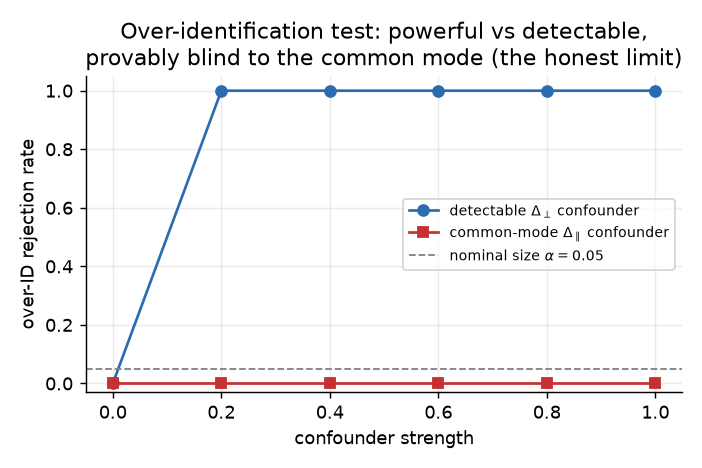
\includegraphics[width=0.49\linewidth]{figures/fig1_overid_size_power.png}
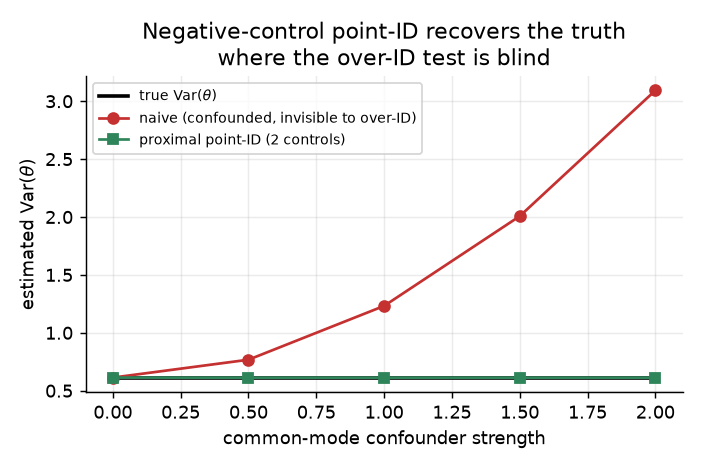
\includegraphics[width=0.49\linewidth]{figures/fig3_proximal_rescue.png}
\caption{\textbf{Left:} the over-identification test is powerful against a
detectable ($\Delta_\perp$) confounder and \emph{provably blind} to a
common-mode ($\Delta_\parallel$) confounder---the honest fundamental limit.
\textbf{Right:} with two negative controls, proximal \emph{point-identification}
recovers the true latent variance where the naive estimate inflates without
bound. Both panels are generated directly from the tested implementation.}
\label{fig:core}
\end{figure}

\begin{figure}[t]
\centering
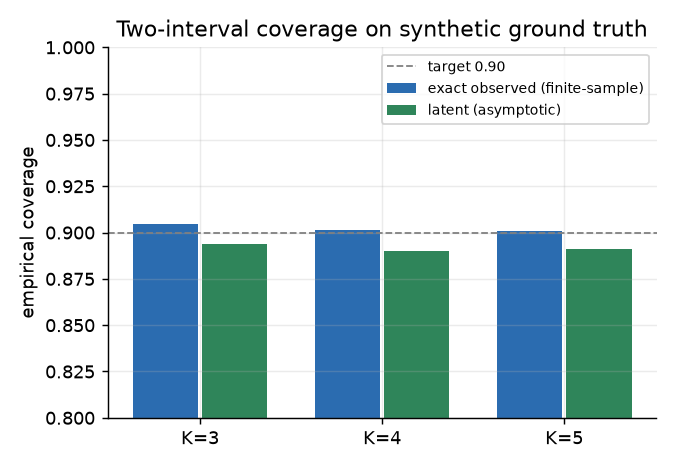
\includegraphics[width=0.49\linewidth]{figures/fig2_coverage.png}
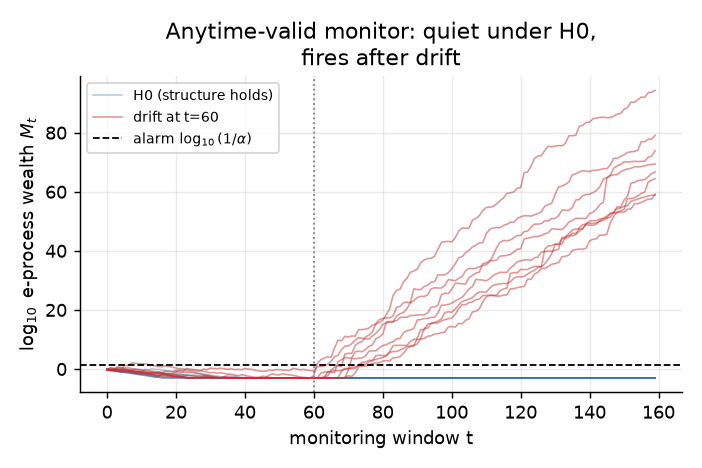
\includegraphics[width=0.49\linewidth]{figures/fig4_monitor.png}
\caption{\textbf{Left:} the two-interval conformal design---an exact
finite-sample interval for the observed pivot value and a model-assisted latent
interval---both near their $0.90$ target across $K$. \textbf{Right:} the
anytime-valid e-process stays quiet under the null (structure holds) and fires
shortly after a drift at $t{=}60$, with a time-uniform $5\%$ false-alarm
guarantee (Ville). Generated from the tested implementation.}
\label{fig:conf_monitor}
\end{figure}

\paragraph{Point-identification, exclusion sensitivity, and monitoring (implemented).}
Beyond the residualization correction, the released code point-identifies the
latent variance from $Q\ge 2$ valid controls via the anchored two-factor
covariance identities: normalizing one control loading, the confounder variance
$\mathrm{Var}(W)$, the signal confounder-loadings $l_c$, and hence a cleaned
covariance $\mathrm{Cov}(Y^c,Y^d)-l_c l_d\,\mathrm{Var}(W)$ are recovered, from
which the ordinary tetrad estimator returns the deconfounded
$\mathrm{Var}(\theta)$ (Fig.~\ref{fig:core}, right; Table~\ref{tab:pointid}),
with a detection gate that avoids spurious correction when no common mode is
present. To answer the untestable-exclusion objection head-on
(Sec.~\ref{sec:exclusion}), we sweep a bounded exclusion violation
$\eps\in[0,\eps_{\max}]$ over both signs and report the implied
$\Var(\theta)$ band \eqref{eq:exclband} and robustness value $\eps^\star$
(Fig.~\ref{fig:exclusion}): the band collapses to the point estimate at
$\eps=0$, widens monotonically with $\eps$, and \emph{contains} the true
$\Var(\theta)$ under a known injected violation---so an analyst reading the band
is never misled about how fragile the point-ID claim is. A deployment monitor
(Fig.~\ref{fig:conf_monitor}, right; Sec.~\ref{sec:monitor}) runs a Vovk--Wang
$p$-to-$e$ calibrated product e-process over the stream of per-period
over-identification $p$-values; by Ville's inequality it controls the
\emph{anytime} false-alarm rate at $\alpha$ (verified $0.013 \le 0.05$ over long
null streams) while detecting a structural drift with median delay $\approx 9$
windows. Every estimator reported here carries a bootstrap (i.i.d.\ or
moving-block) uncertainty band.

\begin{figure}[t]
\centering
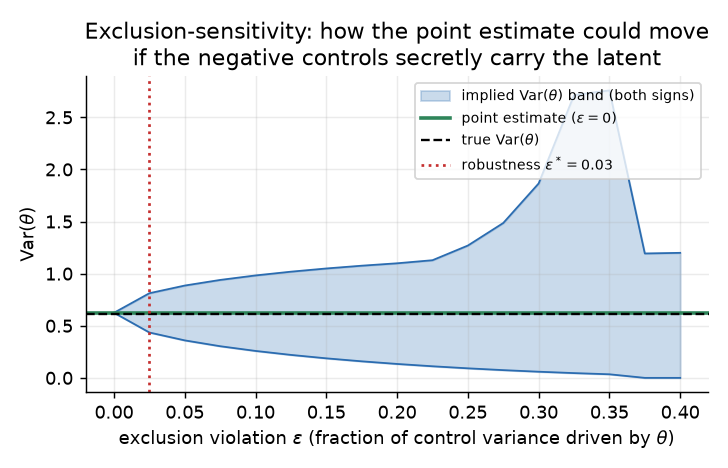
\includegraphics[width=0.6\linewidth]{figures/fig5_exclusion_sensitivity.png}
\caption{\textbf{Exclusion-sensitivity analysis.} As the bounded exclusion
violation $\eps$ (fraction of a control's systematic variance driven by
$\theta$) grows, the implied $\Var(\theta)$ band widens from the proximal point
estimate at $\eps=0$. Sweeping both signs of the (unidentified) violation, the
band \emph{contains} the true $\Var(\theta)$ under a known injected violation;
the robustness value $\eps^\star$ marks where a qualitative conclusion would
flip. This is a bounded bias analysis, not a confidence set: $\eps_{\max}$ is an
expert prior. Generated from the tested implementation.}
\label{fig:exclusion}
\end{figure}

\subsection{Real data: India NCRB, 2001--2010}\label{sec:ncrb}

We apply OICC to India National Crime Records Bureau state-year data,
2001--2010, $N=253$ state-year units, using four institutional channels that
plausibly share a latent ``harm/accountability pressure'' factor while
differing in mechanism:
\begin{enumerate}[leftmargin=1.6em,itemsep=1pt]
\item recorded IPC crime (registration channel);
\item distress calls (citizen-initiated channel);
\item complaints against police (grievance channel);
\item custodial-death and human-rights-violation accountability filings.
\end{enumerate}

\paragraph{Specification.}
The over-ID test does \emph{not} reject the one-factor law in detectable
directions: $p = 0.088$. Per Theorem~\ref{thm:impossible} this does
\emph{not} rule out a common-mode confounder (e.g.\ a state-wide
reporting-culture factor that scales all four channels together); it only
certifies the model against orthogonal misspecification.

\paragraph{Recovered latent.}
The recovered latent ordering is face-valid: large, high-activity states
(Maharashtra, Madhya Pradesh, Andhra Pradesh) rank high; small northeastern
states rank low. We report \emph{no latent coverage number on real data},
because $\theta$ is unobservable there---any such number would be fiction.
This omission is deliberate and, we argue, the honest choice.

\subsection{Cross-national contrast: US crime categories}\label{sec:us}

As a specification-test sanity check we run OICC on real Chicago and NYC panels
(2018--2023), treating the three recorded crime \emph{categories} (violent,
property, drug) as ``channels.'' These share a single police recording filter,
so they are \emph{not} mechanism-independent, and a trustworthy over-ID test
should say so. It does: on both cities the test rejects the one-factor$+$CI
structure at $p<0.001$, in sharp contrast to the India cross-institution
channels ($p{=}0.088$, no rejection). The test thus separates genuinely
independent channels from shared-filter pseudo-channels---validation in both
directions. We do \emph{not} treat crime categories as a latent-victimization
channel set; a real US latent run would require mechanism-independent channels
(records $+$ 911 calls-for-service $+$ NCVS).

%==============================================================
\section{Honest Limitations}\label{sec:limitations}
%==============================================================

\begin{description}[leftmargin=0em,itemsep=3pt]
\item[Common-mode blind spot.] By Theorem~\ref{thm:impossible}, a confounder
loaded along $\beta$ is invisible to any over-ID test and unidentified from
the observed covariance. Without negative controls we can only bound its
effect via the user knob $\gamma_{\text{cm}}$; we cannot estimate it.
\item[Untestable control exclusion.] Proximal correction requires that the
negative controls carry $W$ but not $\theta$, plus completeness. These are
\emph{untestable} (Remark~1). We report naive and proximal estimates side by
side rather than presuppose the assumptions, and---rather than merely
disclaiming---we \emph{bound} the consequence of an exclusion failure with the
exclusion-sensitivity band and robustness value $\eps^\star$ of
Sec.~\ref{sec:exclusion}. This is the honest response to the standard objection
that exclusion cannot be tested: we cannot estimate the violation, but we can
report how far it would have to reach to overturn a conclusion. It remains a
bounded-bias analysis with an expert-supplied $\eps_{\max}$ and an unidentified
violation sign, not a data-driven certainty.
\item[Resolution ceiling.] The latent interval width is floored by the
identified $\Var(S)$; when channels are highly correlated with the pivot,
$\Var(S)$ shrinks but so does the independent information, and at $K=3$ the
over-ID test is powerless (third-cumulant fallback only).
\item[Different constructs.] The one-factor assumption presumes the channels
measure the \emph{same} $\theta$ up to loading. If two channels track
genuinely different constructs (e.g.\ ``violence'' vs.\ ``institutional
distrust''), the recovered factor is a blend; the over-ID test can flag this
\emph{only} to the extent the discrepancy is orthogonal to the dominant
factor.
\end{description}

%==============================================================
\section{Conclusion}\label{sec:conclusion}
%==============================================================

OICC estimates a never-observed latent rate from multiple biased
institutional records and, uniquely, reports what part of that estimate is
defensible. The novelty is the composition and the leave-pivot-out latent
conformal primitive, not any single ingredient: closed-form tetrad
identification, a loading-invariant over-ID test, an exact conformal interval
for a held-out channel plus an asymptotic deconvolution interval for the
latent rate, and an explicit impossibility/escape pairing. We prove and
demonstrate that a common-mode confounder is undetectable and unidentified,
and that negative controls restore identification under honestly untestable
assumptions. On synthetic ground truth every guarantee is met numerically;
on real NCRB data the model survives detectable-direction testing and yields
a face-valid latent ordering, with no fictional latent-coverage claim. We
hope the design principle---return a certificate, not just a number---is
adopted more broadly wherever records are mistaken for truth.

%==============================================================
\appendix
\section*{Appendix: Proofs}
%==============================================================
Full proofs of Propositions~\ref{prop:ident}--\ref{prop:proximal},
Lemma~\ref{lem:indep}, and Theorems~\ref{thm:coverage}--\ref{thm:impossible}
are deferred to the supplementary appendix. Sketches: Prop.~\ref{prop:ident}
follows from \eqref{eq:cov} and the tetrad constraints; Prop.~\ref{prop:power}
and Thm.~\ref{thm:impossible} follow by substituting $\delta=\dperp+\dpar$
into \eqref{eq:logadd} and observing that $\dpar$ rescales all
$\beta_c$ by a common factor absorbed into $c$; Lemma~\ref{lem:indep}
follows from conditional independence in Assumption~\ref{ass:onefactor};
Thm.~\ref{thm:coverage} Interval~1 is standard split-conformal exchangeability,
Interval~2 is a delta-method/deconvolution consistency argument;
Prop.~\ref{prop:proximal} is the proximal identification result of
\cite{miao2018,kurokipearl2014} applied after residualization.

%==============================================================
\begin{thebibliography}{99}
%==============================================================

\bibitem{kotlarski1967}
I.~Kotlarski.
\newblock On characterizing the gamma and the normal distribution.
\newblock \emph{Pacific Journal of Mathematics}, 20(1):69--76, 1967.

\bibitem{livuong1998}
T.~Li and Q.~Vuong.
\newblock Nonparametric estimation of the measurement error model using
multiple indicators.
\newblock \emph{Journal of Multivariate Analysis}, 65(2):139--165, 1998.

\bibitem{huschennach2008}
Y.~Hu and S.~M. Schennach.
\newblock Instrumental variable treatment of nonclassical measurement error
models.
\newblock \emph{Econometrica}, 76(1):195--216, 2008.

\bibitem{dhm2008}
A.~Delaigle, P.~Hall, and A.~Meister.
\newblock On deconvolution with repeated measurements.
\newblock \emph{The Annals of Statistics}, 36(2):665--685, 2008.

\bibitem{miao2018}
W.~Miao, Z.~Geng, and E.~J. Tchetgen Tchetgen.
\newblock Identifying causal effects with proxy variables of an unmeasured
confounder.
\newblock \emph{Biometrika}, 105(4):987--993, 2018.

\bibitem{kurokipearl2014}
M.~Kuroki and J.~Pearl.
\newblock Measurement bias and effect restoration in causal inference.
\newblock \emph{Biometrika}, 101(2):423--437, 2014.

\bibitem{romano2019cqr}
Y.~Romano, E.~Patterson, and E.~J. Cand\`es.
\newblock Conformalized quantile regression.
\newblock In \emph{Advances in Neural Information Processing Systems (NeurIPS)},
2019.

\bibitem{jin2023}
Y.~Jin, Z.~Ren, and E.~J. Cand\`es.
\newblock Sensitivity analysis of individual treatment effects: A robust
conformal inference approach.
\newblock \emph{Proceedings of the National Academy of Sciences (PNAS)},
120(6):e2214889120, 2023.

\bibitem{ppi}
A.~N. Angelopoulos, S.~Bates, C.~Fannjiang, M.~I. Jordan, and T.~Zrnic.
\newblock Prediction-powered inference.
\newblock \emph{Science}, 382(6671):669--674, 2023.

\bibitem{chugg2023}
B.~Chugg, S.~Cortes-Gomez, B.~Wilder, and A.~Ramdas.
\newblock Prediction-powered inference with sequential and adaptive data.
\newblock \emph{arXiv preprint}, 2023.

\bibitem{manriquevallier}
D.~Manrique-Vallier.
\newblock Bayesian population size estimation using Dirichlet process
mixtures.
\newblock \emph{Biometrics}, 72(4):1246--1254, 2016.

\bibitem{cinelli2020}
C.~Cinelli and C.~Hazlett.
\newblock Making sense of sensitivity: Extending omitted variable bias.
\newblock \emph{Journal of the Royal Statistical Society: Series B},
82(1):39--67, 2020.

\bibitem{shi2020}
X.~Shi, W.~Miao, and E.~J. Tchetgen Tchetgen.
\newblock A selective review of negative control methods in epidemiology.
\newblock \emph{Current Epidemiology Reports}, 7:190--202, 2020.

\bibitem{ramdas2023}
A.~Ramdas, P.~Gr\"unwald, V.~Vovk, and G.~Shafer.
\newblock Game-theoretic statistics and safe anytime-valid inference.
\newblock \emph{Statistical Science}, 38(4):576--601, 2023.

\bibitem{wsr2024}
I.~Waudby-Smith and A.~Ramdas.
\newblock Estimating means of bounded random variables by betting.
\newblock \emph{Journal of the Royal Statistical Society: Series B},
86(1):1--27, 2024.

\end{thebibliography}

\end{document}
